%%____________________________________________________________________________||
\section{Physics objects}
\label{sec:objects}
The definitions of the physics objects used in this analysis follow the ongoing recommendations of the various Physics Object Groups (POGs) and PHYS14 subgroup investigations. 

\subsection{Jets}
\label{sec:jetreco}
Jets are defined as sets of particle-flow candidates clustered by the
anti-$k_{T}$ jet clustering algorithm with a distance parameter of 0.4
(PFJets). The Charged Hadron Subtraction (CHS) is applied, i.e., charged
hadrons that can be traced back to pileup vertices are not clustered.
The four-momenta of jets are initially defined as the four-vector sum of
the four-momenta of the constituent particle-flow candidates and then
scaled by the jet energy correction factors designated as L1FastJet,
L2Relative, and L3Absolute.

It should be noted that the early L1 FastJet corrections require
improvements at this stage, and as a result can impact the L2 and L3
corrections. The Tight working point Jet-Id selection criteria was
chosen for the PHYS14 investigation. Figure \ref{fig:QCDJets} shows the
jet resolution in simulation as a function of $p_{T}$, for QCD in the Signal region.

\begin{figure}[h]
  \centering
  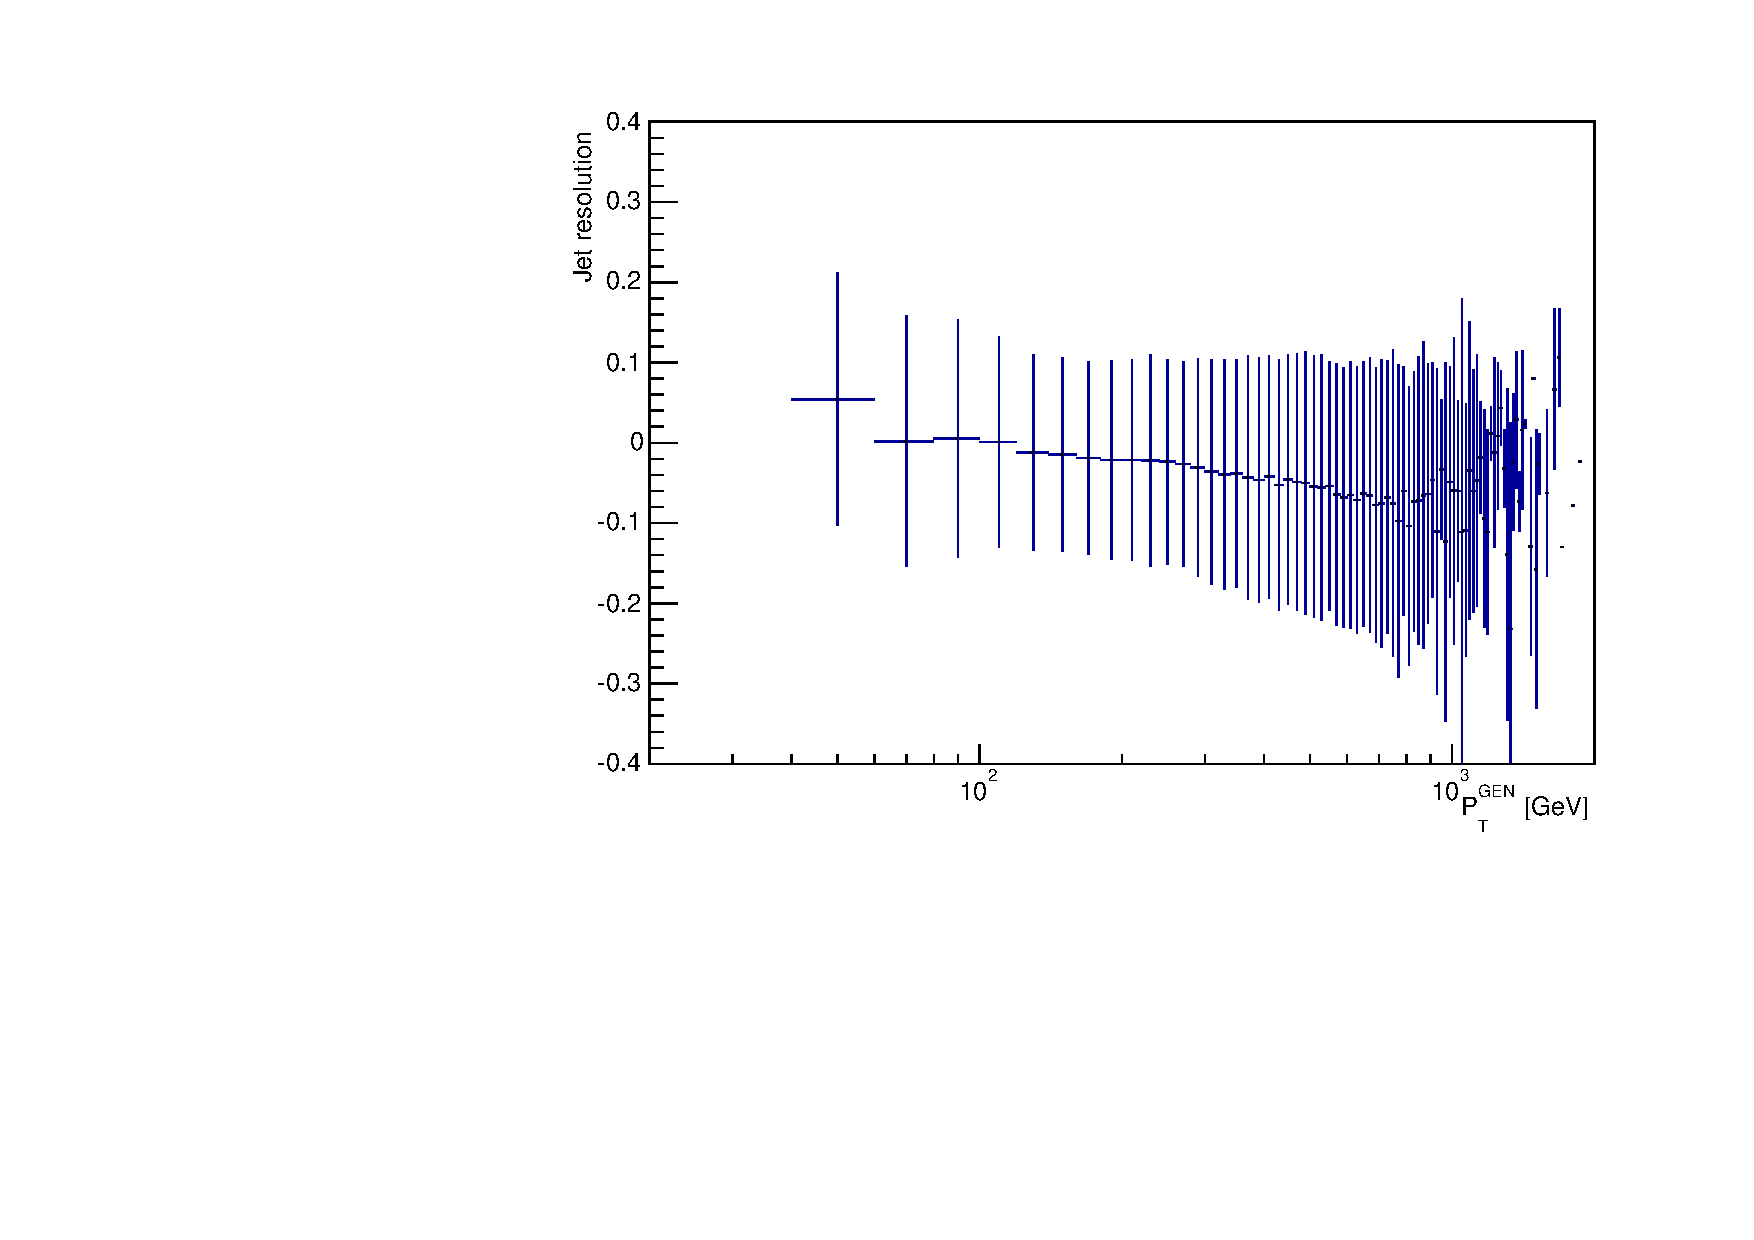
\includegraphics[width=0.6\textwidth]{figures/PhysicsObjectsPlots/JetResolutionSigQCD.pdf}
  \caption{Jet resolution of matched QCD jets in the Signal region}
  \label{fig:QCDJets}
\end{figure}
   
  

\subsection{b-tagged jets}
\label{sec:btags}
Jets originating from bottom quarks are identified through vertices that are displaced with respect to the primary interaction \cite{b-tagging}. The algorithm used to tag b-jets is the Combined Secondary Vertex tagger V2, using the ``Medium`` working point, which is achieved by requiring a cut of $>$ 0.814 on the algorithm discriminator variable and results in a gluon/light-quark mis-tag rate of 1.0623 $\%$ ( where ``light`` means $\it{u}$, $\it{d}$ and $\it{s}$ quarks).



\subsection{Muons}
\label{sec:muon-id}
Muons are identified according to the Tight working point definition ($\sim$ 95 $\%$ efficiency ) of the muon identifiction algorithim. A PF-based ``combined relative`` isolation is determined within a cone size of $\Delta R < 0.4 $, and ``$\rho$``corrections are applied to remove the effects of pileup. Isolated muons are required to have minimal energy from neutral and charged PF candidates. A cone of $\Delta R$ = 0.4 is formed around the candidate lepton trajectory, and the transverse momenta is summed over PF neutral and charged candidates, excluding that of the lepton itself. The relative combined isolation $I^{rel}_{comb}$ is then defined as the ratio of this scalar sum to the transverse momentum of the lepton candidate. 
Figures \ref{fig:SMStack} and \ref{fig:DMStack} show the relative combined isolation $I^{rel}_{comb}$ for $\mu +$ jets and $\mu\mu +$ jets control sample. The distributions have been weighted according to the cross-section of the respective samples in each region, and an integrated luminosity of 1 fb$^{-1}$ at $\sqrt{s}$ = 13 TeV. Isolated muons promptly produced in the decays of W and Z bosons dominate the region $I^{rel}_{comb}$ $<$ 0.12.
In the case of high jet multiplicity events, an increase in energy resulting in boosted events can result in complicated topologies for leptons and jets. For example high $p_{T}$ top quarks decaying leptonically, the main issue is the small angular separation between that of the lepton and the b-jet. Classical lepton isolation techniques will reject the boosted leptonic top quarks. A solution to this is to reduce the cone size around the lepton in function of $p_{T}$. This technique known as Mini Isolation is currently being investigated as a potential candidate for increasing the prompt lepton efficiency in boosted topologies.  

Muons are used as a veto as part of the hadronic signal region definition, as described in Section \ref{sec:hadSelection}, and as part of the $\mu +$ jets and $\mu\mu +$ jets control sample selections as described in Section \ref{sec:controlSelection}.

\begin{figure}[h]
  \centering
  \subfigure[Relative combined isolation variable for \texorpdfstring{\mj}{muon plus jets}
  control sample]{
    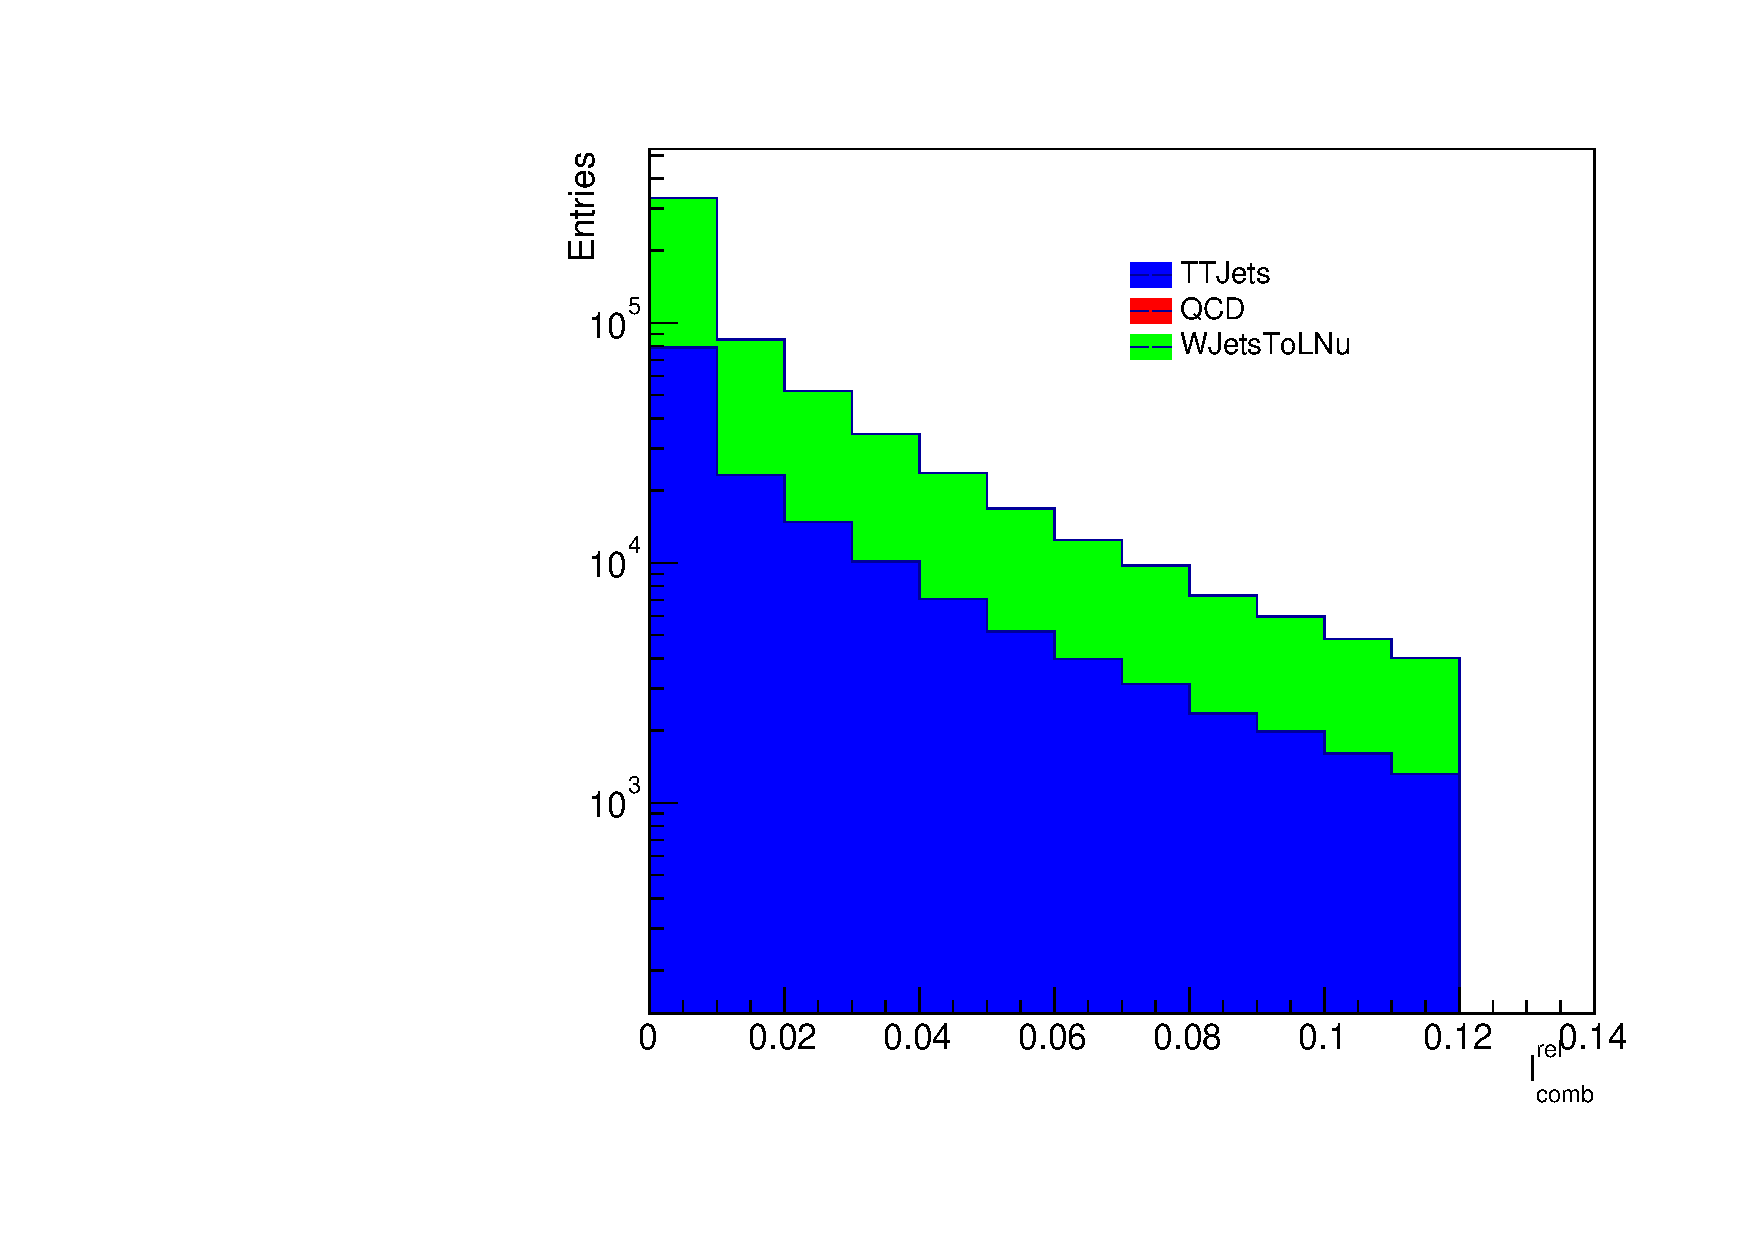
\includegraphics[width=0.5\textwidth]{figures/PhysicsObjectsPlots/SingleMuStack.pdf}
    \label{fig:SMStack}
  }~~
  \subfigure[Relative combined isolation variable for \texorpdfstring{\mmj}{di-muon plus jets}
    control sample]{
    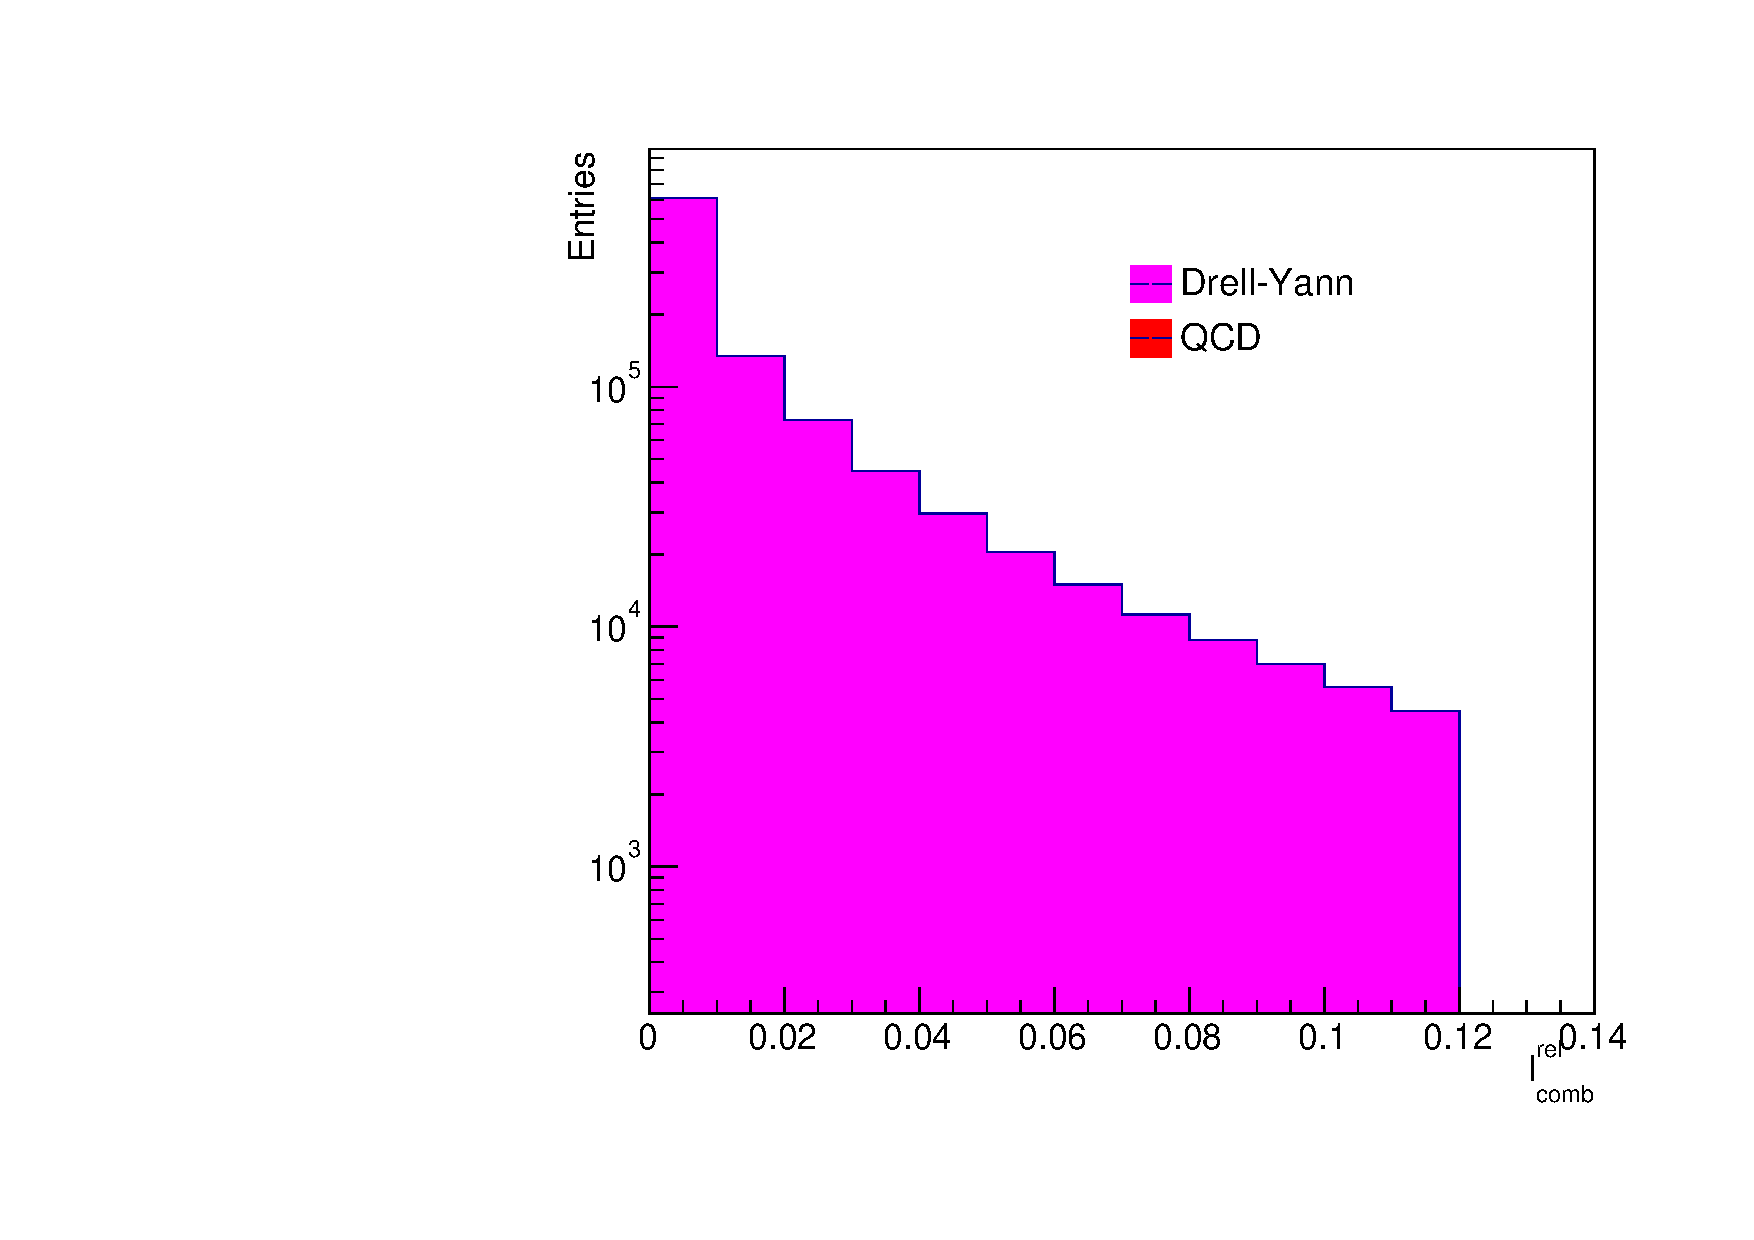
\includegraphics[width=0.5\textwidth]{figures/PhysicsObjectsPlots/DoubleMuStack.pdf}
    \label{fig:DMStack}
  }~~  
\caption{$I_{comb}^{rel}$ for \texorpdfstring{\mj}{muon plus jets} & \texorpdfstring{\mmj}{di-muon plus jets} control samples}
\end{figure}


\subsection{Photons}
\label{sec:photon-id}
Photons are identified according to the Tight working point defintion ($\sim$ 70 $\%$ efficiency) of the simple cut-based photon identification algorithm \cite{photon-id}. PF-based isolation is determined within a cone size $\Delta R$ $<$ 0.3 and $\rho$ x $A_{eff}$ corrections are applied to remove the effects of pileup \cite{pf-photon}. Table \ref{tab:photon-id-gamma} summarises the identification and isolation requirements for PHYS14 samples. 
This object is used as a veto as part of the hadronic signal region definiton, as described in Section \ref{sec:hadSelection}, and as part of the $\gamma$ + jets control sample described in Section \ref{subsec:photoncontrolSelection}.

\begin{table}[ht!]
  \caption{Photon identification (Tight working point).\label{tab:photon-id-gamma}}
  \centering
  \footnotesize
  \begin{tabular}{ ccc }
    \hline
    \hline
    Categories                    & Barrel                             & EndCap                             \\
    \hline
    Conversion safe electron veto & Yes                                & Yes                                \\
    Single Tower H/E              & 0.012                              & 0.011                               \\
    $\sigma_{i\eta i\eta}$        & 0.098                              & 0.0264                               \\
    PF charged hadron isolation   & 1.91                               & 1.26                               \\
    PF neutral hadron isolation   & 2.55 + 0.0023 $\times$ $\pt^{\gamma}$  & 2.71 + 0.0116 $\times$ $\pt^{\gamma}$  \\
    PF photon isolation           & 1.29 + 0.0004 $\times$ $\pt^{\gamma}$ & 1.91 + 0.0037 $\times$ $\pt^{\gamma}$ \\
    \hline
    \hline
  \end{tabular}
  \end{table}


\subsection{Electrons}
\label{sec:electron-id}
Electrons are identified according to the Loose working point definition ( $\sim$ 90 $\%$ efficiency ) of the cut-based identification \cite{electron-id}. PF-based isolation \cite{pf-photon} is determined within a cone size of $\Delta R$ $<$ 0.3 and $\Delta \beta$ corrections are applied to remove the effects of pileup. Table \ref{tab:ele-d} summarises the identification and isolation requirements derived using the PHYS14 samples. 	

\begin{table}[h!]
  \caption{Electron identification (Loose working point).\label{tab:ele-id}}
  \centering
  \footnotesize
  \begin{tabular}{ lcc }
    \hline
    \hline
    Categories                                               & Barrel    & EndCap    \\
    \hline
    $\Delta \eta_{In}$                                       & 0.010557  & 0.010654  \\
    $\Delta \phi_{In}$                                       & 0.012442  & 0.145129  \\
    $\sigma_{i\eta i\eta}$                                   & 0.072624  & 0.032602  \\
    H/E                                                      & 0.121476  & 0.131862  \\
    d0 (vtx)                                                 & 0.022664  & 0.097358  \\
    dZ (vtx)                                                 & 0.173670  & 0.198444  \\
    $\lvert(1/E_{\textrm{ECAL}} - 1/p_{\textrm{trk}})\rvert$ & 0.221803  & 0.142283  \\
    PF relative isolation                                    & 0.120026  & 0.162914  \\
    Missing hits                                             & 1         & 1         \\
    \hline
    \hline
  \end{tabular}
  \end{table}


\subsection{Single Isolated Tracks}
\label{sec:SIT}

A single isolated track (SIT) can be used to identify W bosons through their leptonic decays: W $\rightarrow$ $\mu \nu$, W $\rightarrow$ $e\nu$, and W $\rightarrow$ $\tau$($\rightarrow l$) $\nu$. Single prong decays of the tau lepton can be identified: W $\rightarrow$ $\tau$ ($\rightarrow$ h$^{\pm}$ + n$\pi^{0}$) $\nu$. A single isolated track comprises a charged PF candidate that satisfies the requirements listed in Table \ref{tab:sit-id}. The relative track isolation is determined from the vectorial sum of neighbouring charged PF candidates within a cone $\Delta R$ $<$ 0.3 and satisfying $\Delta$z(candidate, PV) $<$ 0.05cm around the candidate isolated track.
This object can be used to efficiently suppress the ``lost lepton`` background from W and t$\bar{t}$, as described in Section 7.1. 

\begin{table}[h!]
  \caption{Single isolated track identification.\label{tab:sit-id}}
  \centering
  \footnotesize
  \begin{tabular}{ lc }
    \hline
    \hline
    Track \Pt                      & $>10\gev$  \\
    $\Delta z (\textrm{track,PV})$ & $<0.05\cm$ \\
    Charge                         & $\neq 0$   \\
    Relative track isolation       & $<0.1$     \\
    \hline
    \hline
  \end{tabular}
  \end{table}

\subsection{Missing transverse momenum}
Missing transverse momentum is defined as the negative of the vector sum
of the transverse momentum of all particle-flow candidates in the event.
The Type-I MET correction is applied, i.e., the transverse momentum of
the particle-flow candidates clustered as jets are replaced with the
transverse momentum of the jets that are scaled by the jet energy
correction factors \cite{METCorrections}.

The missing transverse momentum is only used in the following two cases:
to define the transverse mass, $M_{T}$, which is in turn used as part of
the selection criteria that define the $\mu +$ jets control sample,
described in \ref{subsec:mucontrolSelection}, and to define a cleaning filter applied after the
$\alpha_{T}$ requirement, as described in Section \ref{sec:selection}.



%%____________________________________________________________________________||
